After carefully executed Stage-I and Stage-II training, in this section, we will design comprehensive experiments to probe the  hypotheses detailed below. With the stated hypotheses, we aim to extend the envelope of existing understanding and contribute novel insights into the domain of image fusion. We expect that the carefully designed experimental procedure will offer a robust platform to scrutinize these hypotheses, shed light on the latent aspects, and help us further refine our model's capability and performance. We will be testing the capabilities of the model into two different approach: capabilities of the new loss function and the model.

\subsection{Study I: New Loss Function}

\begin{table*}[htbp]
    \centering
    % \captionsetup{justification=raggedright, singlelinecheck=false}
    \caption{Loss Functions Comparison}
    \label{tab:ch5:met2}
    \begin{tabular*}{\linewidth}{@{\extracolsep{\fill}}|l|l|l|l|l|}
        \hline
        \textbf{Folder} & \textbf{Entropy\cite{roberts2008assessment}$\uparrow$ } & \textbf{SCD\cite{aslantas2015new}$\downarrow$} & \textbf{MI\cite{qu2002information}$\uparrow$} & \textbf{SSIM\cite{ma2015perceptual}$\uparrow$} \\ \hline
        Proposed $L_{fuse}$ in Eq \ref{eq:fuseloss} & 4.536 & \textbf{5.433} & \textbf{1.591} & \textbf{0.884} \\ \hline
        $L_{ae}$ as $L_{fuse}$ Exp & 4.559 & 6.466 & 0.552 & 0.879 \\ \hline
        RFN-Nest\cite{li2021rfn} & \textbf{4.729} & 7.062 & 0.602 & 0.541 \\ \hline
    \end{tabular*}
\end{table*}

Employing our novel loss function, which prioritizes the similarity between visible and infrared inputs, is anticipated to yield more informative fused images compared to using the Structural Similarity Metric (SSIM). To validate this hypothesis, the proposed loss function (\(L_{fuse}\)) was implemented, emphasizing the preservation of significant features from both input sources. Multiple model versions were trained using different loss functions—one utilizing the traditional SSIM loss and the other employing our newly proposed loss function, with all other parameters held constant for a fair comparison. The evaluation involved qualitative analysis, assessing details, contrast, sharpness, and overall perceptual quality of the fused images, as well as quantitative comparisons using metrics such as \(pSSIM\) and mutual information. By scrutinizing the quality and information retention in the resulting fused images, this comprehensive approach allows us to ascertain the validity of the hypothesis. The newly proposed loss function exhibits commendable abilities in both qualitative and quantitative results, as evident from Figure \ref{fig:ch5:met2} and Table \ref{tab:ch5:met2}. Notably, when evaluated at nearly identical SSIM scores, the loss function proposed in Eq. \ref{eq:fuseloss} demonstrates superior performance compared to the conventionally adopted loss function detailed in Eq. \ref{eq:aeloss}. The inclusion of RFN-Nest results ensures a comprehensive assessment, highlighting the potential of our methodology to outperform traditional standards, especially in terms of the SSIM metric. This comparison underscores the significance of the innovative approach embodied by the newly proposed loss function, offering promising insights and paving the way for advancements in image fusion and related fields.

\begin{figure}[htbp]
    \centering
    \begin{subfigure}[b]{\textwidth}
        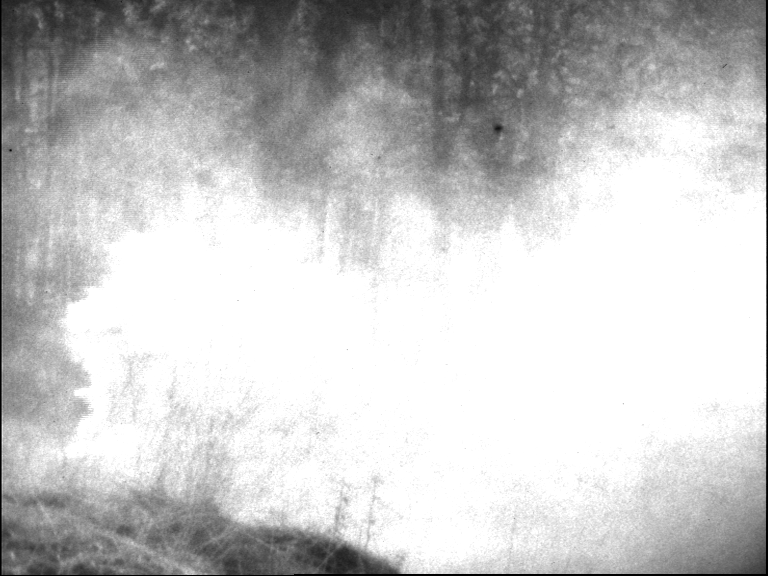
\includegraphics[width=0.16\textwidth, height=0.1\textheight]{imgs/ch5/vis/20.png}
        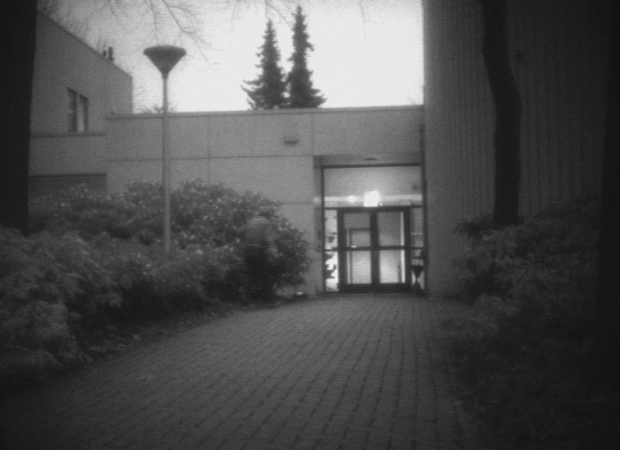
\includegraphics[width=0.16\textwidth, height=0.1\textheight]{imgs/ch5/vis/12.png}
        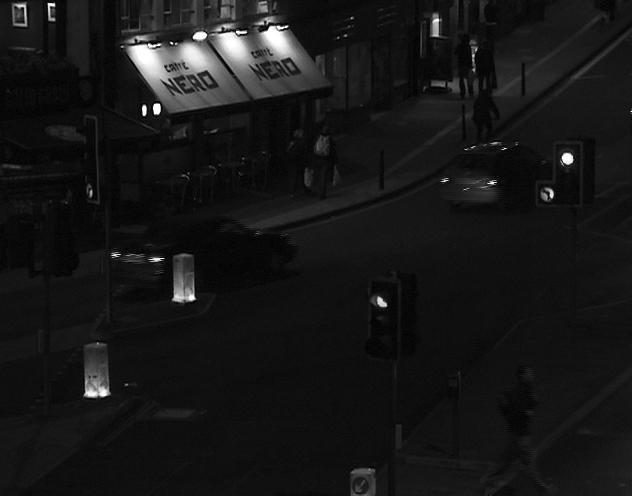
\includegraphics[width=0.16\textwidth, height=0.1\textheight]{imgs/ch5/vis/02.png}
        \captionsetup{justification=raggedright,singlelinecheck=false}
        \caption{Visual Band Images}
        \label{fig:ch5:met2:vis}
    \end{subfigure}
    \vspace{0.01cm}
    \begin{subfigure}[b]{\textwidth}
        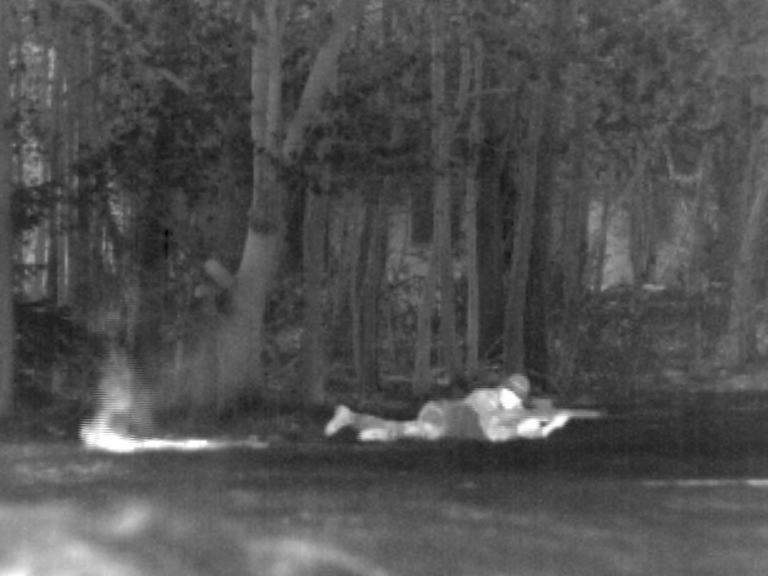
\includegraphics[width=0.16\textwidth, height=0.1\textheight]{imgs/ch5/ir/20.png}
        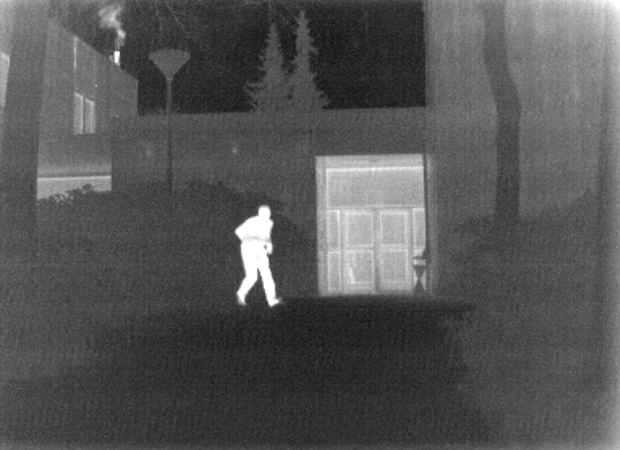
\includegraphics[width=0.16\textwidth, height=0.1\textheight]{imgs/ch5/ir/12.png}
        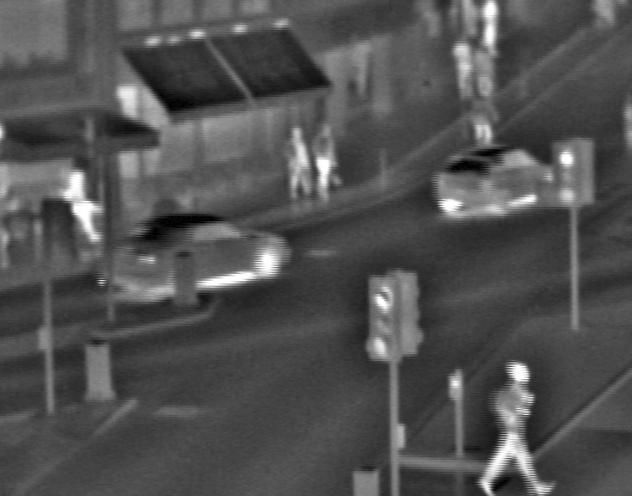
\includegraphics[width=0.16\textwidth, height=0.1\textheight]{imgs/ch5/ir/02.png}
        \captionsetup{justification=raggedright,singlelinecheck=false}
        \caption{Infrared Band Images}
        \label{fig:ch5:met2:ir}
    \end{subfigure}
    \vspace{0.01cm}
    \begin{subfigure}[b]{\textwidth}
        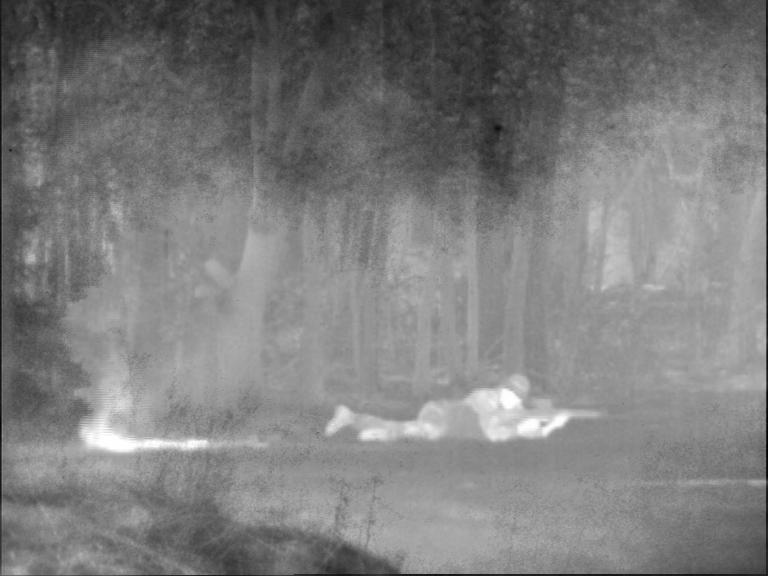
\includegraphics[width=0.16\textwidth, height=0.1\textheight]{imgs/ch5/ours/20.jpg}
        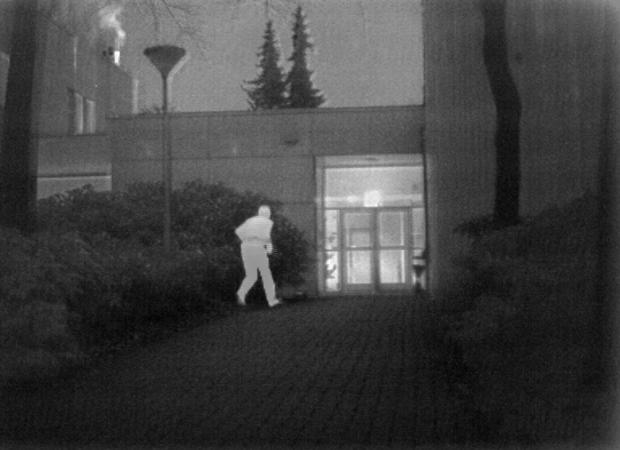
\includegraphics[width=0.16\textwidth, height=0.1\textheight]{imgs/ch5/ours/12.jpg}
        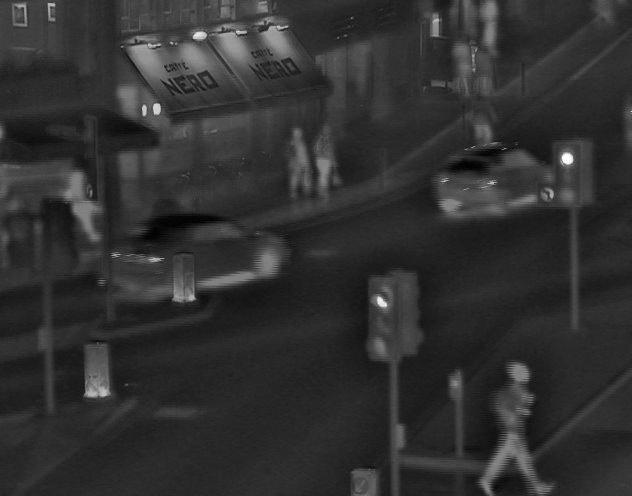
\includegraphics[width=0.16\textwidth, height=0.1\textheight]{imgs/ch5/ours/02.jpg}
        \captionsetup{justification=raggedright,singlelinecheck=false}
        \caption{Model With New $L_{fuse}$ Loss Output Images}
        \label{fig:ch5:met2:ours}
    \end{subfigure}
    \vspace{0.01cm}
    \begin{subfigure}[b]{\textwidth}
        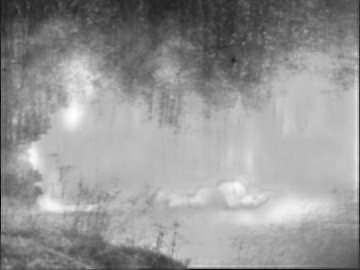
\includegraphics[width=0.16\textwidth, height=0.1\textheight]{imgs/ch5/sameLoss/20.png}
        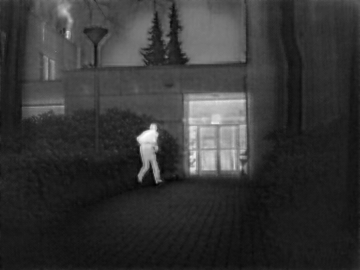
\includegraphics[width=0.16\textwidth, height=0.1\textheight]{imgs/ch5/sameLoss/12.png}
        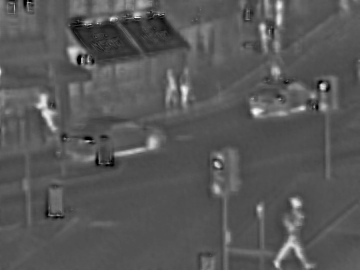
\includegraphics[width=0.16\textwidth, height=0.1\textheight]{imgs/ch5/sameLoss/02.png}
        \captionsetup{justification=raggedright,singlelinecheck=false}
        \caption{Model With $ L_{fuse} = L_{ae}$ Loss Output Images}
        \label{fig:ch5:met2:sameLoss}
    \end{subfigure}
    \captionsetup{justification=raggedright,singlelinecheck=false}
        \caption{Loss Functions Comparison}
    \label{fig:ch5:met2}
\end{figure}

The comparison our model with leading image fusion methods are given in Figure \ref{fig:ch5:met4}. We'll evaluate them based on visual quality and the quantitative metrics. As highlighted in Section \ref{chp:RelatedWork}, current top methods include transformer-based techniques like M3FD\cite{liu2022target} and IFT\cite{vs2022image}, GAN-based approaches such as DenseFuse\cite{li2019infrared} and SwinFusion\cite{ma2022swinfusion}, and the autoencoder method RFN-Nest\cite{li2021rfn}. Our goal is to provide a clear and thorough comparison to understand the strengths and limitations of each method in the field of image fusion.

\begin{figure}[htbp]
    \centering
    \begin{subfigure}[b]{\textwidth}
        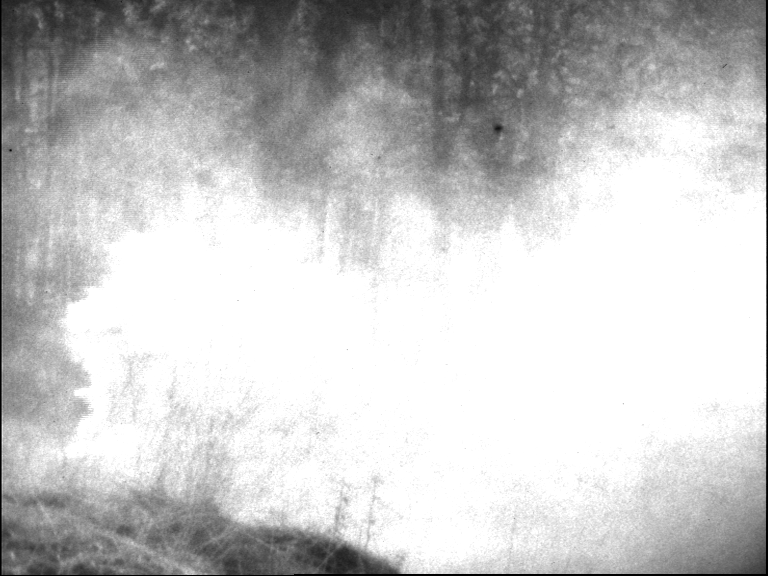
\includegraphics[width=0.16\textwidth, height=0.1\textheight]{imgs/ch5/vis/20.png}
        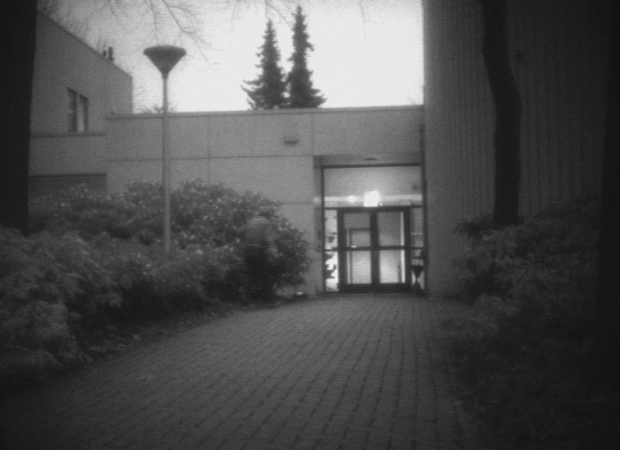
\includegraphics[width=0.16\textwidth, height=0.1\textheight]{imgs/ch5/vis/12.png}
        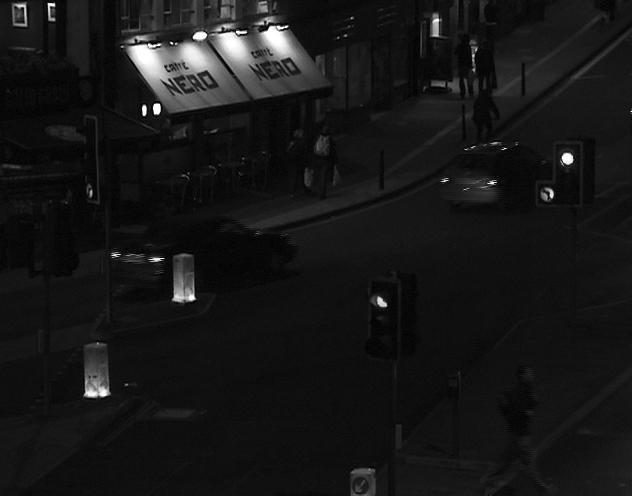
\includegraphics[width=0.16\textwidth, height=0.1\textheight]{imgs/ch5/vis/02.png}
        \captionsetup{justification=raggedright,singlelinecheck=false}
        \caption{Visual Band Images}
        \label{fig:ch5:met9:vis}
    \end{subfigure}
    \vspace{0.01cm}
    \begin{subfigure}[b]{\textwidth}
        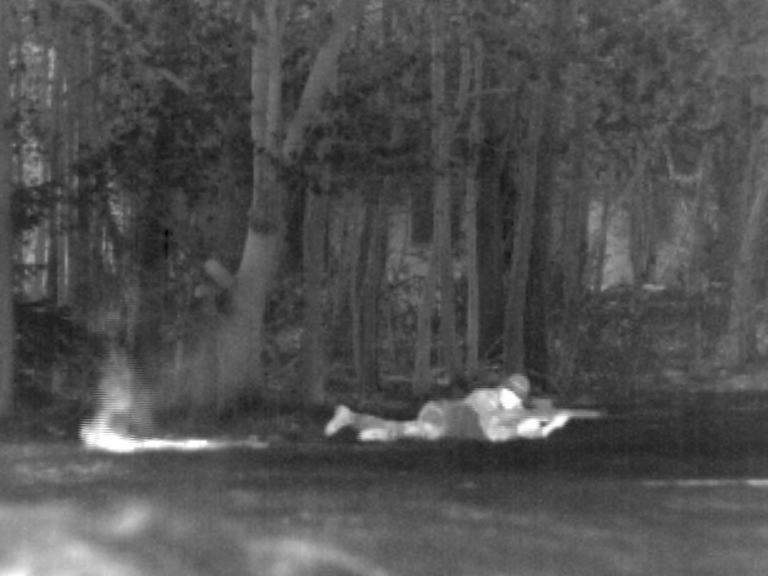
\includegraphics[width=0.16\textwidth, height=0.1\textheight]{imgs/ch5/ir/20.png}
        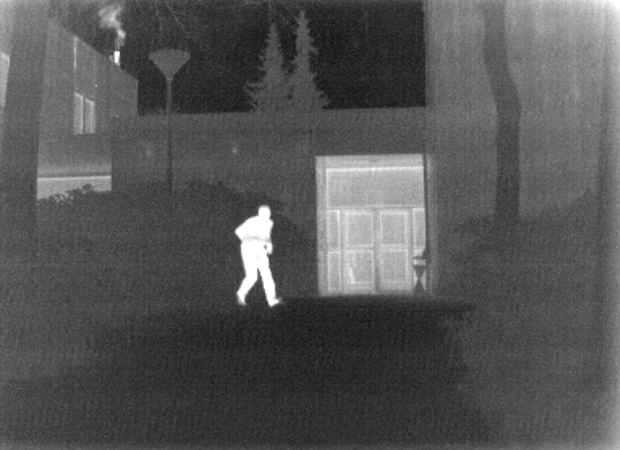
\includegraphics[width=0.16\textwidth, height=0.1\textheight]{imgs/ch5/ir/12.png}
        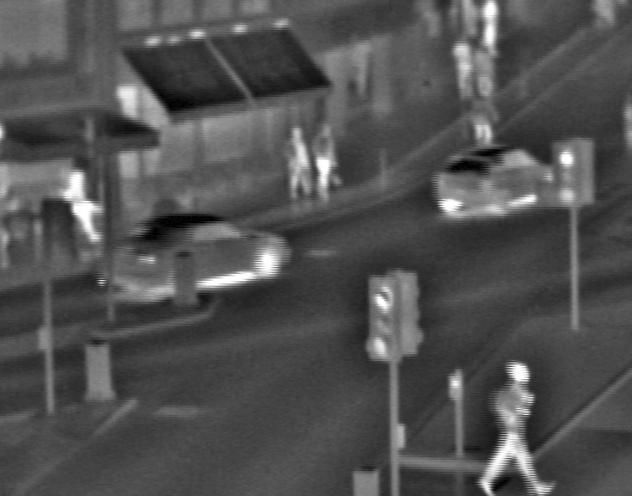
\includegraphics[width=0.16\textwidth, height=0.1\textheight]{imgs/ch5/ir/02.png}
        \captionsetup{justification=raggedright,singlelinecheck=false}
        \caption{Infrared Band Images}
        \label{fig:ch5:met9:ir}
    \end{subfigure}
    \vspace{0.01cm}
    \begin{subfigure}[b]{\textwidth}
        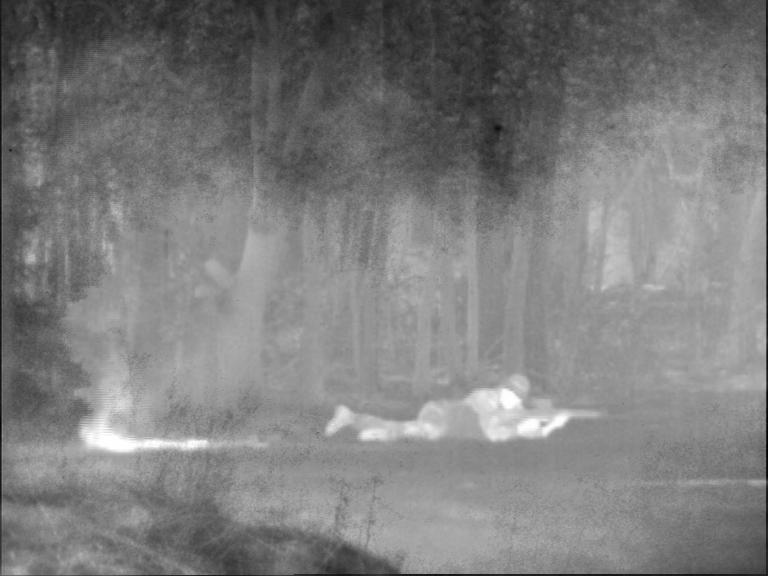
\includegraphics[width=0.16\textwidth, height=0.1\textheight]{imgs/ch5/ours/20.jpg}
        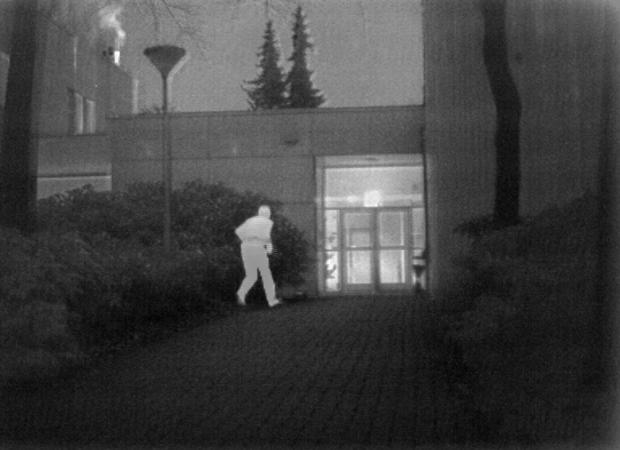
\includegraphics[width=0.16\textwidth, height=0.1\textheight]{imgs/ch5/ours/12.jpg}
        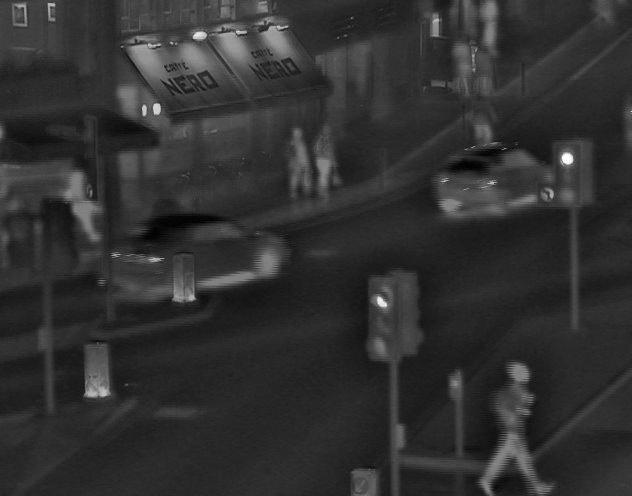
\includegraphics[width=0.16\textwidth, height=0.1\textheight]{imgs/ch5/ours/02.jpg}
        \captionsetup{justification=raggedright,singlelinecheck=false}
        \caption{Our Output Images}
        \label{fig:ch5:met9:ours}
    \end{subfigure}
    \vspace{0.01cm}
    \begin{subfigure}[b]{\textwidth}
        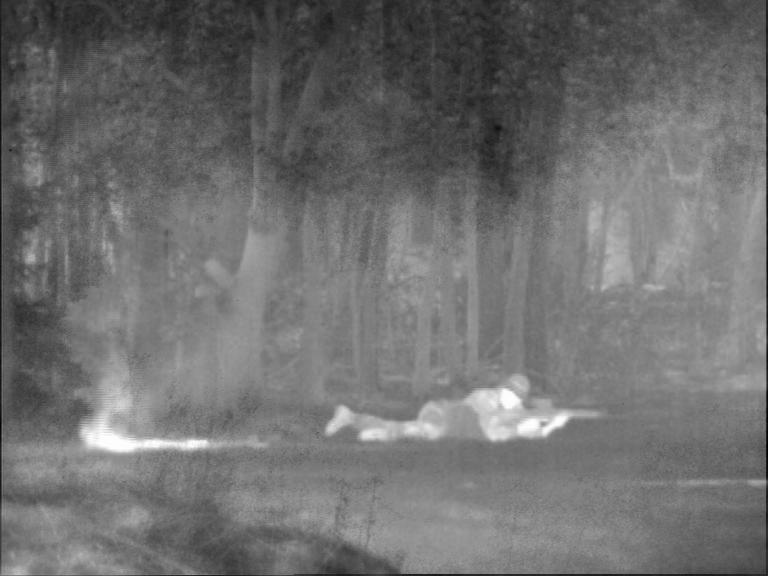
\includegraphics[width=0.16\textwidth, height=0.1\textheight]{imgs/ch5/swinFusion/20.jpg}
        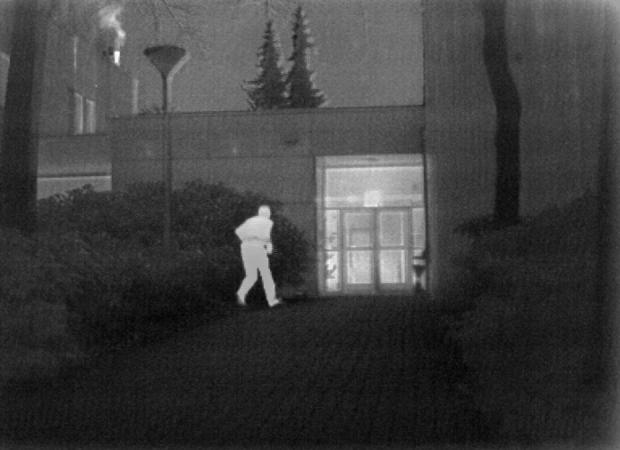
\includegraphics[width=0.16\textwidth, height=0.1\textheight]{imgs/ch5/swinFusion/12.jpg}
        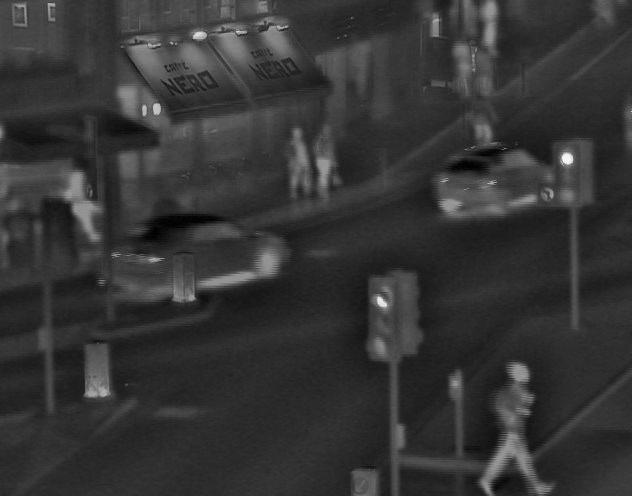
\includegraphics[width=0.16\textwidth, height=0.1\textheight]{imgs/ch5/swinFusion/02.jpg}
        \captionsetup{justification=raggedright,singlelinecheck=false}
        \caption{SwinFusion\cite{ma2022swinfusion} Output Images}
        \label{fig:ch5:met9:swin}
    \end{subfigure}
    \captionsetup{justification=raggedright,singlelinecheck=false}
        \caption{Comparison with SoTA}
    \label{fig:ch5:met4}
\end{figure}

\begin{figure}[htbp]
    \centering
    \begin{subfigure}[b]{\textwidth}
        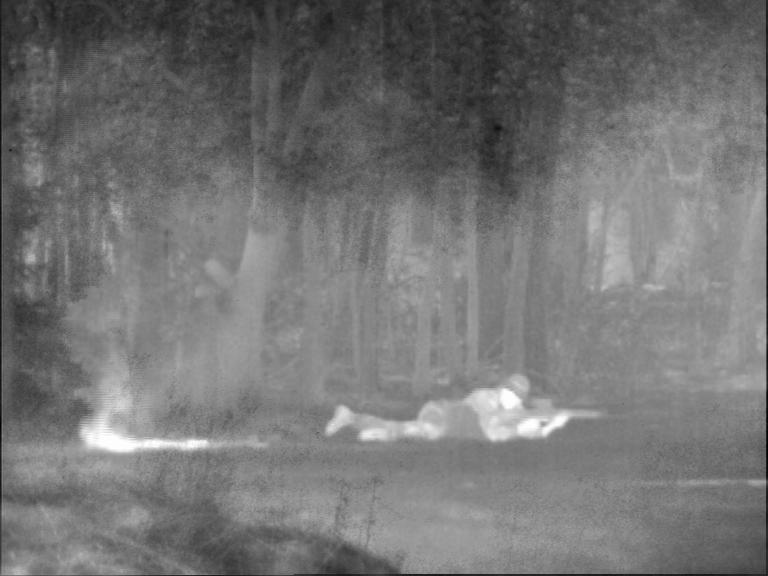
\includegraphics[width=0.16\textwidth, height=0.1\textheight]{imgs/ch5/m3fd/20.jpg}
        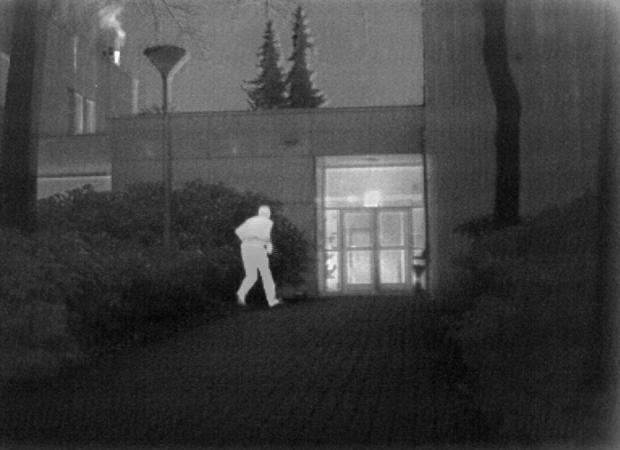
\includegraphics[width=0.16\textwidth, height=0.1\textheight]{imgs/ch5/m3fd/12.jpg}
        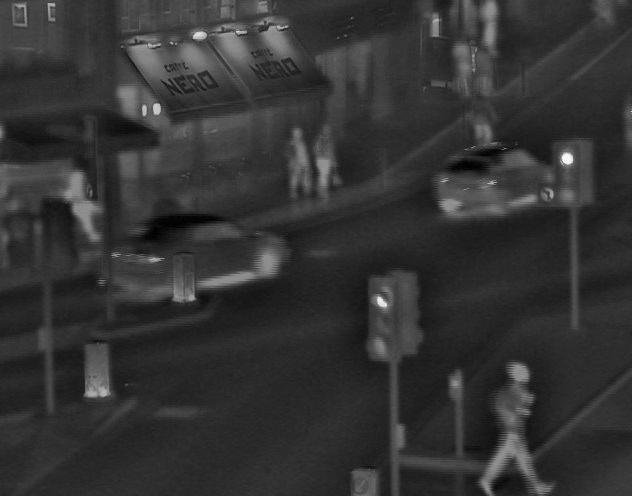
\includegraphics[width=0.16\textwidth, height=0.1\textheight]{imgs/ch5/m3fd/02.jpg}
        \captionsetup{justification=raggedright,singlelinecheck=false}
        \caption{M3FD\cite{liu2022target} Output Images}
        \label{fig:ch5:met9:m3fd}
    \end{subfigure}
    \vspace{0.01cm}
    \begin{subfigure}[b]{\textwidth}
        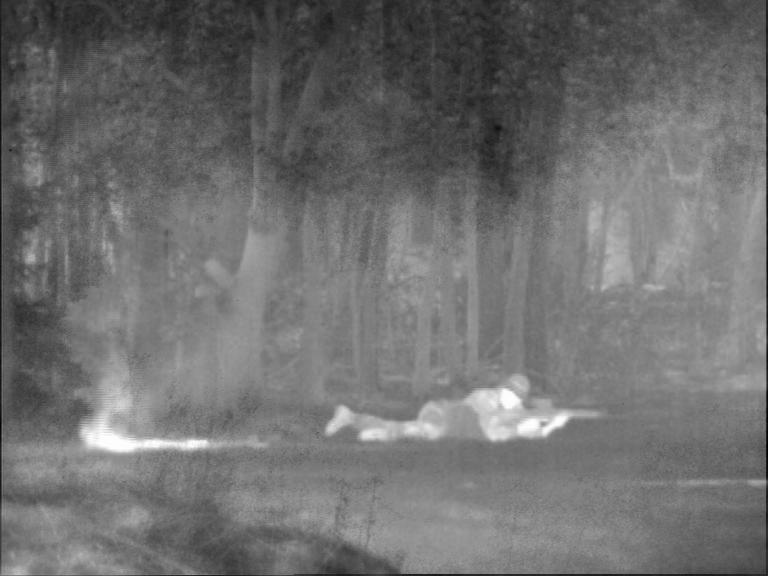
\includegraphics[width=0.16\textwidth, height=0.1\textheight]{imgs/ch5/swinFusion/20.jpg}
        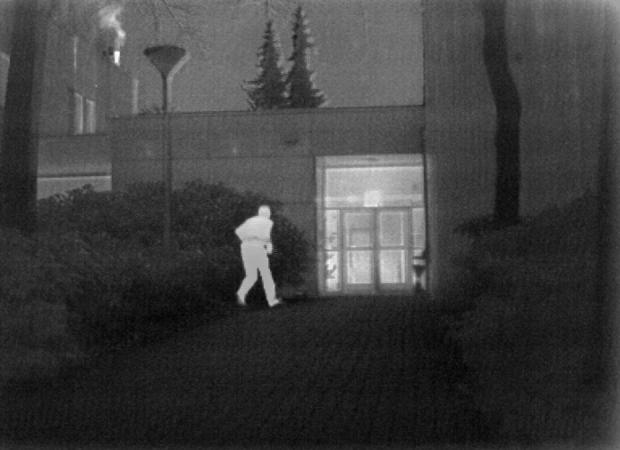
\includegraphics[width=0.16\textwidth, height=0.1\textheight]{imgs/ch5/swinFusion/12.jpg}
        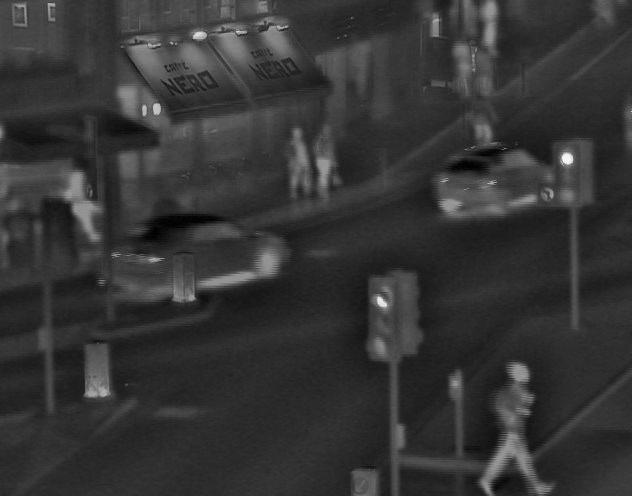
\includegraphics[width=0.16\textwidth, height=0.1\textheight]{imgs/ch5/swinFusion/02.jpg}
        \captionsetup{justification=raggedright,singlelinecheck=false}
        \caption{IFT\cite{vs2022image} Output Images}
        \label{fig:ch5:met9:ift}
    \end{subfigure}
    \vspace{0.01cm}
    \begin{subfigure}[b]{\textwidth}
        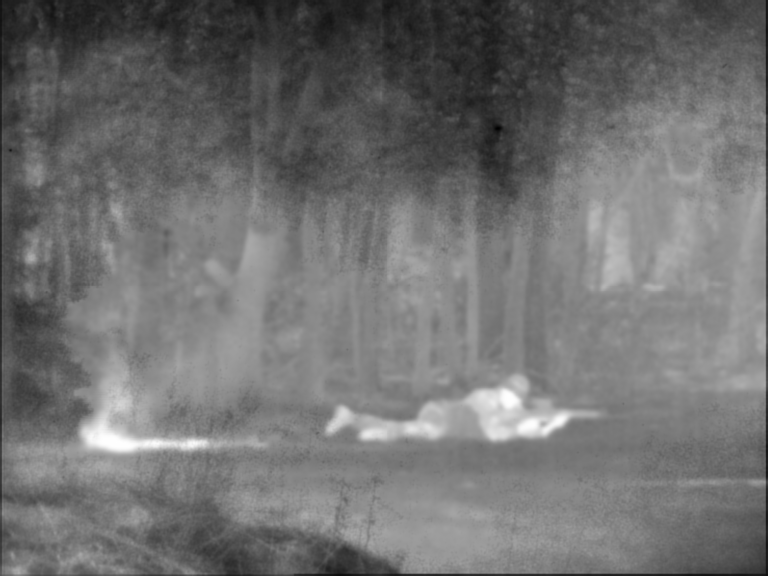
\includegraphics[width=0.16\textwidth, height=0.1\textheight]{imgs/ch5/rfn/20.png}
        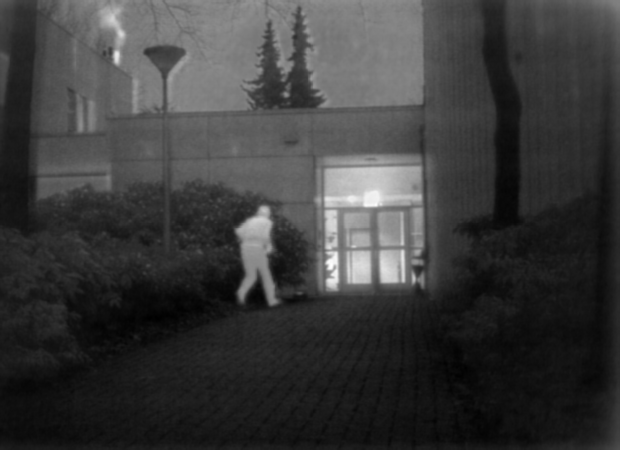
\includegraphics[width=0.16\textwidth, height=0.1\textheight]{imgs/ch5/rfn/12.png}
        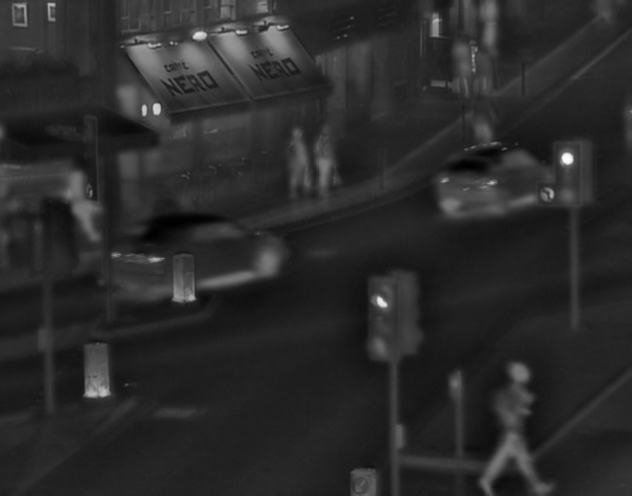
\includegraphics[width=0.16\textwidth, height=0.1\textheight]{imgs/ch5/rfn/02.png}
        \captionsetup{justification=raggedright,singlelinecheck=false}
        \caption{RFN-Nest\cite{li2021rfn} Output Images}
        \label{fig:ch5:met9:rfn}
    \end{subfigure}
    \vspace{0.01cm}
    \begin{subfigure}[b]{\textwidth}
        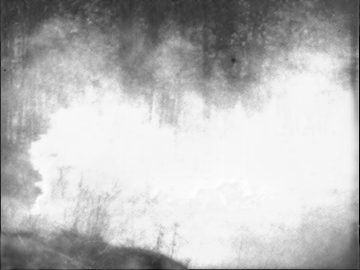
\includegraphics[width=0.16\textwidth, height=0.1\textheight]{imgs/ch5/denseFuse/20.png}
        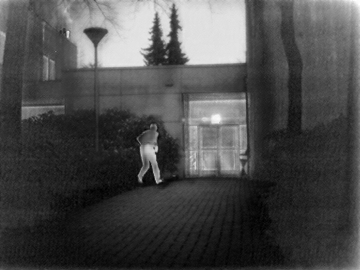
\includegraphics[width=0.16\textwidth, height=0.1\textheight]{imgs/ch5/denseFuse/12.png}
        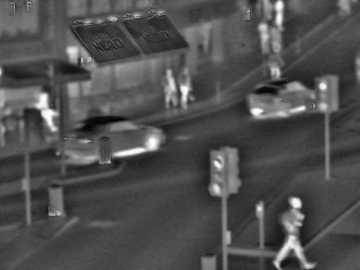
\includegraphics[width=0.16\textwidth, height=0.1\textheight]{imgs/ch5/denseFuse/02.png}
        \captionsetup{justification=raggedright,singlelinecheck=false}
        \caption{DenseFuse\cite{li2019infrared} Output Images}
        \label{fig:ch5:met9:densefuse}
    \end{subfigure}
    \captionsetup{justification=raggedright,singlelinecheck=false}
        \caption{Comparison with SoTA \textit{cont'd}}
\end{figure}

Upon a qualitative assessment of Figure \ref{fig:ch5:met5}, several observations come to the fore. The first column distinctly showcases the imaging of a soldier amidst smoke, and this rendition, with its meticulous portrayal of the surrounding details, stands qualitatively superior to its counterparts. A similar superiority can be discerned in the second column, where the depiction of the man concealed behind the tree is accentuated by the intricate details of the tree's broader context, setting it apart from other state-of-the-art methods presented. The final column further underscores the prowess of our method. Here, one can distinctly discern the brand name on a shop awning and identify pedestrians on the street, all the while maintaining the fidelity of details from the original visual band images. Turning our attention to Table \ref{tab:ch5:met8}, it becomes evident that our method eclipses others in performance across almost all metrics. The sole exception is the \textbf(Entropy\cite{roberts2008assessment}) metric. It's worth noting that entropy gauges the degree to which pixel values in an image are non-redundant. Consequently, original infrared images, as depicted in Figure \ref{fig:ch5:met2:ir}, would naturally register the highest entropy scores. This distinction provides a nuanced understanding of where and how our method stands in relation to others in the domain.

\begin{table*}[htbp]
    \centering
    % \captionsetup{justification=raggedright, singlelinecheck=false}
    \caption{Comparison with SoTA}
    \label{tab:ch5:met8}
    \begin{tabular*}{\linewidth}{@{\extracolsep{\fill}}|l|l|l|l|l|}
        \hline
        \textbf{Method} & \textbf{Entropy\cite{roberts2008assessment}$\uparrow$ } & \textbf{SCD\cite{aslantas2015new}$\downarrow$} & \textbf{MI\cite{qu2002information}$\uparrow$} & \textbf{SSIM\cite{ma2015perceptual}$\uparrow$} \\ \hline
        Ours            & 4.536                & \textbf{5.433}       & \textbf{1.591}           &\textbf{0.884}             \\ \hline
        SwinFusion\cite{ma2022swinfusion}           & 4.605                & 6.760       & 0.804           & 0.690             \\ \hline
        M3FD\cite{liu2022target}           & 4.625                & 6.858       & 0.742           & 0.659             \\ \hline
        IFT\cite{vs2022image}           & 4.644                & 6.864       & 0.684           & 0.630             \\ \hline
        DenseFuse\cite{li2019infrared}           & 4.724                & 6.455       & 0.853           & 0.588             \\ \hline
        RFN-Nest\cite{li2021rfn}            & \textbf{4.729}                & 7.062       & 0.602           & 0.541             \\ \hline
    \end{tabular*}
\end{table*}

\subsection{Study II: A Unique Transformer Based Fusion Strategy}\label{sec:study1}

In this part, our research explores the application of transformer-based models for visual and infrared image fusion, focusing on autoencoders for feature extraction and representation learning. Rooted in hypotheses, our study aims to enhance night vision, medical imaging, and surveillance tasks (\textbf{Hypothesis II-1}), achieve a balance between quantitative and qualitative performance (\textbf{Hypothesis II-2}), demonstrate computational efficiency for real-time applications (\textbf{Hypothesis II-3}), and address challenges through model tuning and regularization (\textbf{Hypothesis II-4}). Our proposed approach combines autoencoder-derived features from visual and infrared images using a transformer-based model, aiming to balance performance and efficiency. Experiments, conducted on the TNO dataset, evaluate these hypotheses, covering diverse tasks and assessments. Results will yield insights into the effectiveness and efficiency of transformer-based image fusion techniques, advancing our understanding in this domain.

\begin{figure}[htbp]
    \centering
    \begin{subfigure}[b]{\textwidth}
        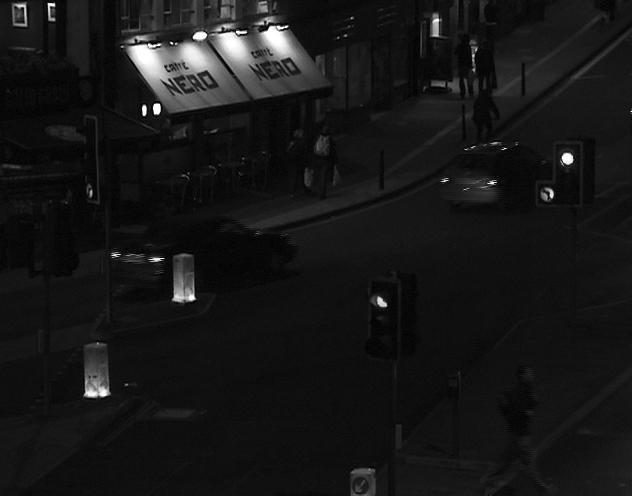
\includegraphics[width=0.16\textwidth, height=0.1\textheight]{imgs/ch5/vis/02.png}
        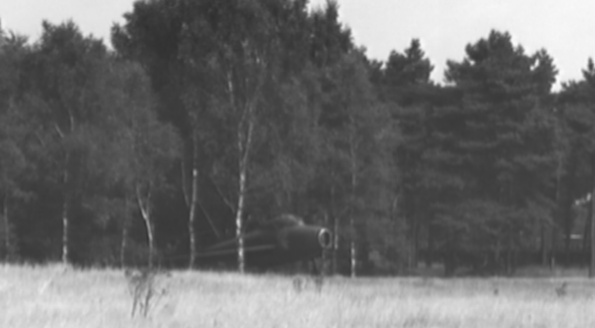
\includegraphics[width=0.16\textwidth, height=0.1\textheight]{imgs/ch5/vis/07.png}
        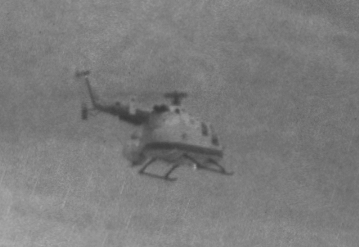
\includegraphics[width=0.16\textwidth, height=0.1\textheight]{imgs/ch5/vis/11.png}
        \captionsetup{justification=raggedright,singlelinecheck=false}
        \caption{Visual Band Images}
        \label{fig:ch5:met4:vis}
    \end{subfigure}
    \vspace{0.01cm}
    \begin{subfigure}[b]{\textwidth}
        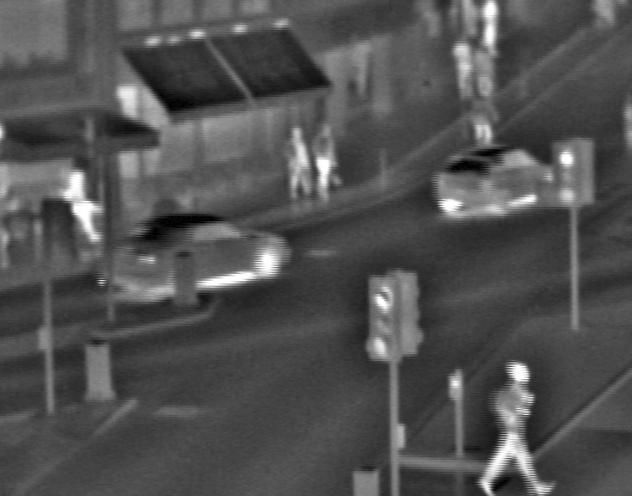
\includegraphics[width=0.16\textwidth, height=0.1\textheight]{imgs/ch5/ir/02.png}
        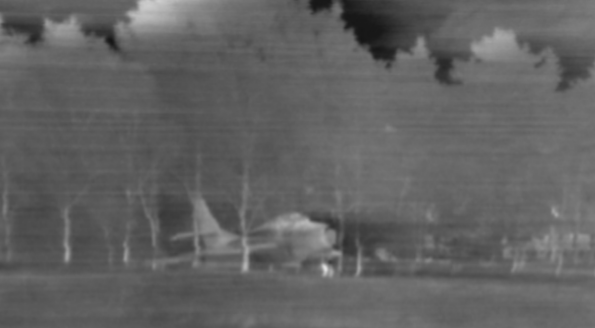
\includegraphics[width=0.16\textwidth, height=0.1\textheight]{imgs/ch5/ir/07.png}
        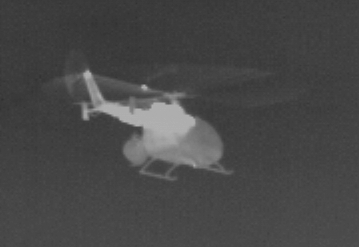
\includegraphics[width=0.16\textwidth, height=0.1\textheight]{imgs/ch5/ir/11.png}
        \captionsetup{justification=raggedright,singlelinecheck=false}
        \caption{Infrared Band Images}
        \label{fig:ch5:met4:ir}
    \end{subfigure}
    \vspace{0.01cm}
    \begin{subfigure}[b]{\textwidth}
        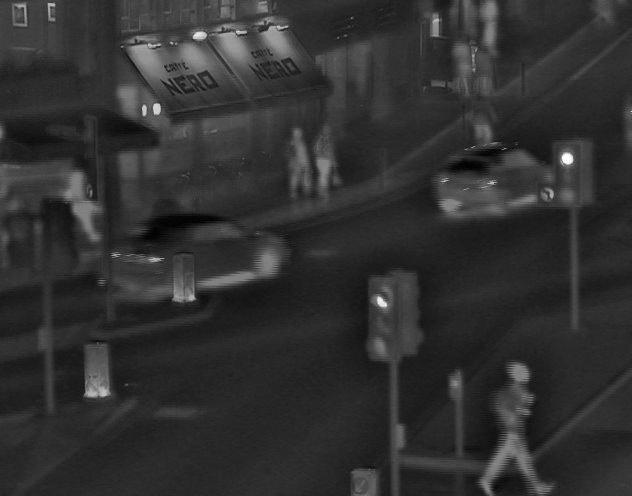
\includegraphics[width=0.16\textwidth, height=0.1\textheight]{imgs/ch5/ours/02.jpg}
        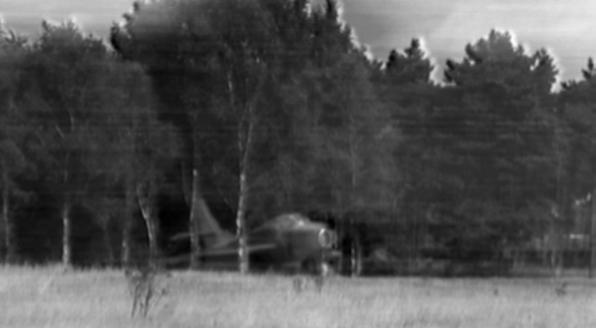
\includegraphics[width=0.16\textwidth, height=0.1\textheight]{imgs/ch5/ours/07.jpg}
        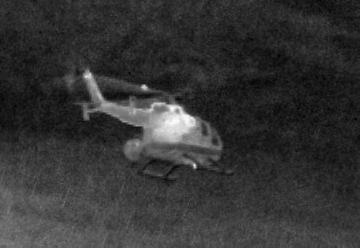
\includegraphics[width=0.16\textwidth, height=0.1\textheight]{imgs/ch5/ours/11.jpg}
        \captionsetup{justification=raggedright,singlelinecheck=false}
        \caption{Our Output Images}
        \label{fig:ch5:met4:ours}
    \end{subfigure}
    \vspace{0.01cm}
    \begin{subfigure}[b]{\textwidth}
        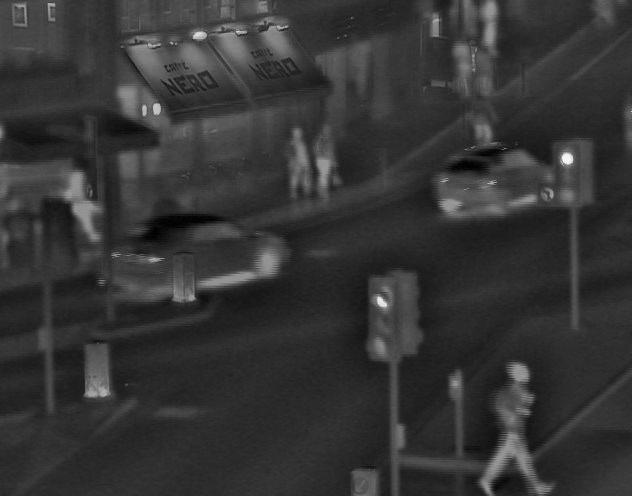
\includegraphics[width=0.16\textwidth, height=0.1\textheight]{imgs/ch5/swinFusion/02.jpg}
        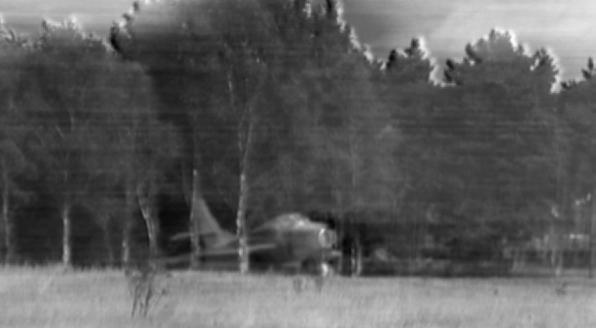
\includegraphics[width=0.16\textwidth, height=0.1\textheight]{imgs/ch5/swinFusion/07.jpg}
        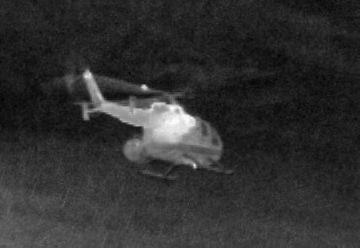
\includegraphics[width=0.16\textwidth, height=0.1\textheight]{imgs/ch5/swinFusion/11.jpg}
        \captionsetup{justification=raggedright,singlelinecheck=false}
        \caption{SwinFusion\cite{ma2022swinfusion}Output Images}
        \label{fig:ch5:met4:swin}
    \end{subfigure}
    \captionsetup{justification=raggedright,singlelinecheck=false}
        \caption{Night Vision Enhancement}
    \label{fig:ch5:met4}
\end{figure}

\begin{figure}[htbp]
    \centering
    \begin{subfigure}[b]{\textwidth}
        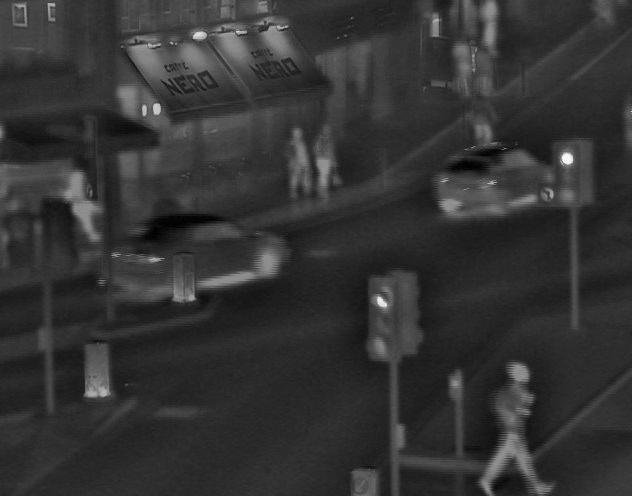
\includegraphics[width=0.16\textwidth, height=0.1\textheight]{imgs/ch5/m3fd/02.jpg}
        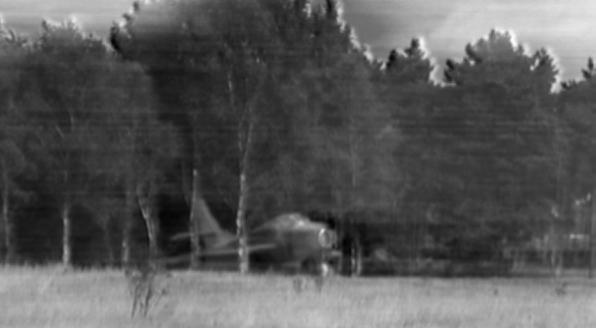
\includegraphics[width=0.16\textwidth, height=0.1\textheight]{imgs/ch5/m3fd/07.jpg}
        \includegraphics[width=0.16\textwidth, height=0.1\textheight]{imgs/ch5/m3fd/11.jpg}
        \captionsetup{justification=raggedright,singlelinecheck=false}
        \caption{M3FD\cite{liu2022target} Output Images}
        \label{fig:ch5:met4:m3fd}
    \end{subfigure}
    \vspace{0.01cm}
    \begin{subfigure}[b]{\textwidth}
        \includegraphics[width=0.16\textwidth, height=0.1\textheight]{imgs/ch5/swinFusion/02.jpg}
        \includegraphics[width=0.16\textwidth, height=0.1\textheight]{imgs/ch5/swinFusion/07.jpg}
        \includegraphics[width=0.16\textwidth, height=0.1\textheight]{imgs/ch5/swinFusion/11.jpg}
        \captionsetup{justification=raggedright,singlelinecheck=false}
        \caption{IFT\cite{vs2022image} Output Images}
        \label{fig:ch5:met4:ift}
    \end{subfigure}
    \vspace{0.01cm}
    \begin{subfigure}[b]{\textwidth}
        \includegraphics[width=0.16\textwidth, height=0.1\textheight]{imgs/ch5/rfn/02.png}
        \includegraphics[width=0.16\textwidth, height=0.1\textheight]{imgs/ch5/rfn/07.png}
        \includegraphics[width=0.16\textwidth, height=0.1\textheight]{imgs/ch5/rfn/11.png}
        \captionsetup{justification=raggedright,singlelinecheck=false}
        \caption{RFN-Nest\cite{li2021rfn} Output Images}
        \label{fig:ch5:met4:rfn}
    \end{subfigure}
    \vspace{0.01cm}
    \begin{subfigure}[b]{\textwidth}
        \includegraphics[width=0.16\textwidth, height=0.1\textheight]{imgs/ch5/denseFuse/02.png}
        \includegraphics[width=0.16\textwidth, height=0.1\textheight]{imgs/ch5/denseFuse/07.png}
        \includegraphics[width=0.16\textwidth, height=0.1\textheight]{imgs/ch5/denseFuse/11.png}
        \captionsetup{justification=raggedright,singlelinecheck=false}
        \caption{DenseFuse\cite{li2019infrared} Output Images}
        \label{fig:ch5:met4:densefuse}
    \end{subfigure}
    \captionsetup{justification=raggedright,singlelinecheck=false}
        \caption{Night Vision Enhancement \textit{cont'd}}
\end{figure}

From Figure \ref{fig:ch5:met4}, the first column showcases an instance of night vision imagery. This particular example serves as a suitable representation for illustrating long-range dependencies and the global context inherent in such images. The second and third columns, on the other hand, predominantly depict scenarios captured under low light conditions. While at a qualitative glance, the distinctions between the images might appear subtle, a closer examination reveals nuanced differences. Turning our attention to Table \ref{tab:ch5:met4}, a comprehensive evaluation indicates that our proposed method consistently delivers superior results. In comparison to state-of-the-art (SoTA) techniques, our method exhibits marked improvements across nearly every evaluated performance metric.

